\part{IDE}

IDE\ --- Integrated Development Environment, интегрированная среда разработки.

Программный пакет, включающий 
\begin{itemize}
  \item средства управления проектом,
  \item отслеживание зависимостей между файлами (в т.ч. с анализом исходного
  текста программ на конструкции типа \verb|#include|, \verb|module|,
  \verb|uses|),
  \item автозапуском компиляторов для изменившихся файлов,
  \item GUI для отладчиков (gdb),
  \item специализированный редактор plain text\note{файлы не включающие
  непечатаемых символов и бинарных данных, которые можно причитать простым
  выводом на экран командами типа \textbf{type}, \textbf{cat}, \textbf{more}}
  файлов c
  \begin{itemize}
    \item цветовой и шрифтовой \term{подстветкой синтаксиса},
  	\item \term{автодополнением}: дописываются имена объектов программ, 
  	синтаксические конструкции и параметры функций,
  	\item \term{автоформатированием}: фрагмент текста переформатируется в
  	соответствии с синтаксисом языка редактируемого файла, проставляются отступы в
  	зависимости от вложенности синтаксических конструкций типа циклов и условных
  	блоков)
  	\item выделением строк, на которые указывают сообщения об ошибках
  	компиляторов,
  	\item маркеры точек останова отладчика
  \end{itemize}
  \item отображение структуры программ, например деревья классов и структур
  данных
  \item контекстные справочники по используемым языкам программирования,
  автоматический вывод списка параметров при вводе имени функции
  \item отображение дизассемблерных листингов для компилируемых языков
  \item отображение браузера как вкладки или MDI окна
  \item отображение вывода \term{статических анализаторов} программ c
  кликабельными ссылками
  \item вывод компиляторов и трансляторов с цветовым выделением и переход на
  ошибочную строку в редакторе при щелчке на ошибке
  \item \ldots
\end{itemize}

В этой книге рассмотрены три бесплатных мультиплатформенных OpenSource IDE, в
порядке навороченности, универсальности, и требуемым ресурсам для работы самой
среды:

\begin{enumerate}
  \item \eclipse\ \ref{eclipse}: самая навороченная и ресурсоемкая IDE, написана
  на Java, имеет десятки дополнительных модулей на все случаи, умеет работать со
  всеми распространенными языками программирования, жрет память, и требует
  современного компьютера минимум с 2+ Гб ОЗУ. Последний релиз \eclipse\ Luna
  работает заметно быстрее (особенно при запуске). 
  \item Code::Blocks \ref{cb}: легкая среда для разработки на C/\cpp, для других
  языков модет потребоваться написать свои модули или файлы описания синтаксиса
  \item Vim \ref{vim}: самый легкий и \emph{портабельный} универсальный
  текстовый редактор с расширенными функциями, работает на всех
  существующих платформах (кроме совсем уж embedded), использует минимум
  ресурсов, но требует некоторого обучения даже чтобы выйти из \verb|vim|
  \smiley
\end{enumerate}

\secrel{\eclipse}\label{eclipse}\secdown


\includegraphics[height=0.5\textheight]{logo/eclipse.png}

\secrel{Установка \eclipse\ под \win}

\menu{\winr>\url{https://eclipse.org/}>Download>Eclipse Luna release for>\win}

Качаем архив базовой системы:
\menu{Eclipse IDE for Java Developers>\win\ 32/64 Bit}

Или сразу сборку CDT\eclipse:
\menu{Eclipse IDE for C/C++ Developers>\win\ 32/64 Bit}

\secrel{Установка \eclipse\ под \linux}

\menu{\winr>\url{https://eclipse.org/}>Download>Eclipse Luna release for>\linux}

Качаем архив базовой системы:
\menu{Eclipse IDE for Java Developers>\linux\ 32/64 Bit}

Или сразу сборку CDT\eclipse:
\menu{Eclipse IDE for C/C++ Developers>\linux\ 32/64 Bit}

\bigskip

Пока качается, параллельно устанавливаем в систему Java-рантайм:

\begin{verbatim}
sudo aptitude install openjdk-7-jre
\end{verbatim}

Распаковывем полученный архив
\file{eclipse-java-luna-SR1-linux-gtk-x86\_64.tar.gz}
в \file{\$HOME}:

\begin{verbatim}
cd ~
tar zx < Downloads/eclipse-java-luna-SR1-linux-gtk-x86_64.tar.gz
ls -la eclipse/eclipse
-rwxr-xr-x 1 user user 74675 Авг 13 16:12 eclipse/eclipse
\end{verbatim}

Прописываем запуск \eclipse\ в ваш оконный менеджер или \file{.blackboxmenu}
с параметром \file{-noSplash} для лечения глюка с запуском на x64-битных
системах:

\lst{.blackbox.menu}{}{ide/eclipse_blackbox.menu}

\secrel{Установка CDT}

\href{https://eclipse.org/cdt/}{\prog{CDT}}\ --- расширение \eclipse\ для
разработки на Си/\cpp, редактирования make-файлов. Это расширение критически
важно для вашей работы, поэтому ставить его обязательно, или сразу качать сборку
CDT\eclipse.
\bigskip

\menu{\eclipse>Help>Install New Software\ldots}

\menu{Work with>Add>Add repository}

\menu{Name>CDT}

\menu{Location>\url{http://download.eclipse.org/tools/cdt/releases/8.5}}

\menu{OK}

\menu{Work with>CDT}

\menu{CDT Main Features>\checkbox\ C/C++ Development Tools}

\menu{CDT Optional Features}

Парсер файлов исходников на диалекте С99:
\menu{\checkbox\ C99 LR Parser}

Поддержка \prog{gcc}\ в режиме кросс-компиляции:
\menu{\checkbox\ GCC Cross Compiler Support}

Аппаратная отладка через \prog{gdb}:
\menu{\checkbox\ GDB Hardware Debugging}

\menu{Next>Next>Accept>Finish}

\secrel{Установка PyDev}

\href{http://pydev.org/}{\prog{PyDev}}\ --- расширение для разработки на Python:
\bigskip

\menu{\eclipse>Help>Install New Software\ldots}

\menu{Work with>Add>Add repository}

\menu{Name>PyDev}

\menu{Location>\url{http://pydev.org/updates}}

\menu{OK}

\menu{Work with>PyDev}

\menu{PyDev>\checkbox\ PyDev for Eclipse}

\menu{Next>Next>Accept>Finish>Certitificate>Restart Eclipse>Ok}

\secrel{Установка TeXlipse}

Если планируете работать с документацией в формате \LaTeX, установите расширение
\href{http://texlipse.sourceforge.net/}{\prog{TeXlipse}}:
\bigskip

\menu{\eclipse>Help>Install New Software\ldots}

\menu{Work with>Add>Add repository}

\menu{Name>TeXlipse}

\menu{Location>\url{http://texlipse.sourceforge.net/}}

\menu{OK}

\menu{Work with>TeXlipse}

Это расширение поддерживает подсветку синтаксиса, автодополнение, построение
динамического оглавления, автокомпиляцию по сохранению, и несколько визардов
создания проекта.

\secrel{Редактирование файлов в формате XML и производных}

Установите пакет \eclipse\ WST:

\menu{Help>Install New Software}

\menu{Work with:>Luna - http://download.eclipse.org/releases/luna}

\menu{Filter:>WST>Eclipse WST>Next>Next>Restart>OK}

\secrel{Проверка орфографии}

\cp{http://www.simplecoding.org/proverka-orfografii-v-eclipse.html}

То, что проверка орфографии очень удобная вещь вряд ли нужно объяснять. Есть
конечно люди, которые не обращают на неё внимание, но это чаще всего из-за
экономии времени и отсутствия удобных средств проверки.

Действительно, удобная автоматическая проверка орфографии есть в офисных
пакетах, но мне сложно представить разработчика, который будет переносить
комментарии в Word и обратно \smiley.

Поэтому очень удобно иметь \emph{проверку правописания прямо в IDE}. И \eclipse\
в этом смысле полностью соответствует ожиданиям.

Долго объяснять что к чему нет смысла. Проверка орфографии встроена в \eclipse\
и если вы пишите только на английском, то может быть не захотите ничего менять.

Кроме того, есть
\href{http://www.102degrees.com/blog/2007/07/09/spell-checking-in-eclipse-pdt/}{статья
Aaron'а} (en) в которой автор рассказывает о подключении дополнительных словарей
и плагине \file{eSpell}.

Но \emph{русских словарей в дистрибутиве нет}, а при подключении внешних есть
нюансы. Поэтому мы максимально подробно рассмотрим \emph{подготовку и добавление
русских словарей}.

Первый вопрос. В каком виде должны быть словари и где их взять?

Тут всё просто. Формат словаря\ --- обычный текстовый файл, в котором каждое
слово начинается с новой строки. И нам вполне подойдут свободно распространяемые
словари \file{aSpell}.

Установка состоит из \ref{aspellecl}\ шагов:
\begin{enumerate}
  \item качаем \href{}{aSpell}\ и словари для нужных языков

  \menu{\winr>\url{http://aspell.net/win32/}>}

  \menu{Binaries>Full installer}

  \menu{Precompiled dictionaries>English}

  \menu{Precompiled dictionaries>Russian}

  \item устанавливаем сначала \file{aSpell}, потом отдельно каждый словарь

  \menu{\file{Aspell-0-50-3-3-Setup.exe}>Setup GNU Aspell>Next>License>Next}

  \menu{Directory>\file{C:/GnuWin32/Aspell}>Next>Next}

  \menu{Additional>Next>Install>Next>\uncheckbox\ View manual>Finish}

  \menu{\file{Aspell-en-0.50-2-3.exe}>Aspell English Dictionary>Next>License>Next}

  \menu{Directory>\file{C:/GnuWin32/Aspell}>Next>Next>Install>Finish}

  \menu{\file{Aspell-ru-0.50-2-3.exe}>Aspell Russian Dictionary>Next>License>Next}

  \menu{Directory>\file{C:/GnuWin32/Aspell}>Next>Next>Install>Finish}

  \item делаем дамп словарей, перекодируем из koi8r в utf8 и объединяем

  \menu{\winr cmd}

\begin{lstlisting}
cd \GnuWin32\Aspell
bin\aspell dump master en > en.dict
bin\aspell dump master ru > ru.koi8
iconv -f koi8-r -t utf-8 < ru.koi8 > ru.dict
copy en.dict + ru.dict enru.dict
\end{lstlisting}

  \item \label{aspellecl} настраиваем \emph{spell-checker} \eclipse

  \menu{\eclipse>Window>Preferences>Editors>Text editors>Spelling}

  \menu{User defined dictionary>\file{C:/GnuWin32/Aspell/enru.dict}}

  \menu{Encoding>UTF-8}

  \menu{Apply>OK}

\end{enumerate}

\secup

\secrel{\cb}\label{cb}\secdown
\secup

\chapter{\vim}\label{vim}


\includegraphics[width=0.3\textwidth]{logo/vim.png}

\section{Установка под \win}

\menu{\winr cmd > \url{http://www.vim.org/} > Download > PC: MS-DOS and
MS-Windows > \href{ftp://ftp.vim.org/pub/vim/pc/gvim74.exe}{\file{gvim74.exe}}}

\menu{Vim 7.4 Setup>This will install>Да}

\menu{License>I'm Angry}

\menu{Installation Options>\checkbox\ Create .bat files>Next}

\menu{Installation Folder>Install}

\menu{Completed>Close}

\menu{Do you want to see README>\textbf{Да}}
\bigskip

Теперь можно настроить темную тему и выключение подстветки синтаксиса, по
умолчанию после установки используется светлая тема и подстветка выключена:

\nopagebreak
\menu{меню>Правка>Настройка запуска}
\bigskip

Переходим в конец файла и включаем \emph{режим вставки}

\keys{Ctrl+Down}\ \keys{Ins}\ \keys{Enter}\keys{Enter}

\begin{lstlisting}
syntax on
colorscheme pablo
\end{lstlisting}
\bigskip

Выходим в \emph{режим команд} и принудительно сохраняем

\keys{Esc}:\keys{w}\keys{!}\keys{Enter}\keys{Enter}
\bigskip

\textbf{Выходим из \vim}

\keys{Esc}:\keys{q}\keys{!}\keys{Enter}

\bigskip
Если не получилось (под Windows 7):

\bigskip
\menu{\winr cmd > \file{/Program Files (x86)/Vim/}}
\bigskip

Копируем файл \file{\_vimrc}\ в любой каталог, например в \file{/tmp/},
затем \menu{\rms\rms>Edit with Vim}, и повторяем редактирование еще раз.

\bigskip
Затем копируем \file{\_vimrc}\ обратно в \file{/Program Files (x86)/Vim/}\ с
заменой.

\bigskip
Если теперь открыть на редактирование тот же файл, или любой другой текстовый,
получим более удобный вид: для файлов известных типов будет работать подсветка
синтаксиса.

\nopagebreak\bigskip
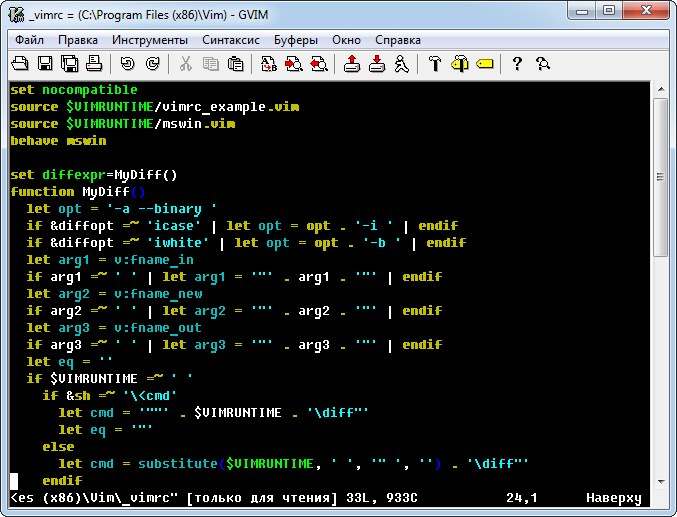
\includegraphics[height=0.9\textheight]{ide/vim28.png}

\section{Выход из \vim}

\keys{Esc}\ :\ \keys{!}\ \keys{q}\ \keys{Enter}

\subsection{Выход с автосохранением}

\keys{Esc}\ \keys{Shift+Z}\ \keys{Shift+Z}

\section{Переход в режим редактирования}

\vim\ запускается в \emph{командном режиме}, для перехода в режим редактирования
используются следующие клавиатурные команды:

\begin{itemize}
  \item \keys{Ins}\ или \keys{i}: включение \emph{режима вставки} по текущему
  положению курсора
  \item \keys{Ins}\keys{Ins}\ или \keys{r}: включение \emph{режима перезаписи}
  поверх текста после курсора
  \item \keys{Shift+A}: включение режима вставки \emph{в конец текущей строки}
\end{itemize}

\section{Переход в режим команд}

\keys{Esc}

\section{Запись редактируемого файла}

\keys{Esc}\ :\ \keys{w}\ \keys{Enter}
\bigskip

Если выводится предупреждение типа ``файл защищен от записи'' или подобное,
может сработать принудительная запись:

\bigskip
\keys{Esc}\ :\ \keys{!}\ \keys{w}\ \keys{Enter}

\section{Перезагрузка файла}

Для перезагрузки возможно изменененного извне файла или отмены всех
несохраненных изменений

\bigskip
\keys{Esc}\ :\ \keys{e}\ \keys{Enter}

\section{Отмена последних изменений (undo)}

\keys{Esc}\keys{u}\keys{u}\ldots

